\chapter{Prototyping in Office Message System}

\section{System description}
The system involves subscribers, publishers and different topics, as to show the workings of the connext middleware. 

\begin{center}
	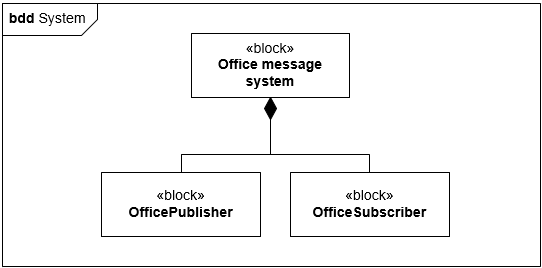
\includegraphics[width=\textwidth]{bdd_image.png}
	\captionof{figure}{BDD of the Office Message System}
\end{center}

The office message system is shown in figure 4.1. The system consists of two different classes, the OfficePublisher and the OfficeSubscriber. The specific topic, type and Quality Of Service of the Subscribers/Publishers are determined through constructor injection.

The prototype will consist of two programs running side by side. One will spawn the subscribers and the other will spawn the publishers. All Readers and Writers are configured for sending messages by the string type. 

The configuration is setup as seen in figure 4.2.

\begin{center}
	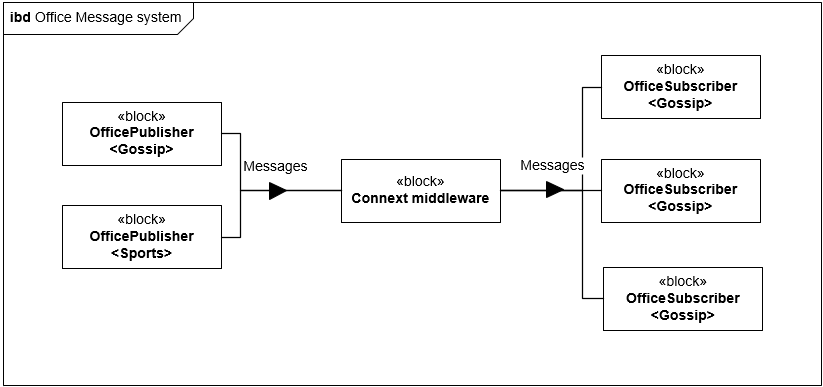
\includegraphics[width=\textwidth]{ibd_image.png}
	\captionof{figure}{IBD of the Office Message System}
\end{center}

As is seen, a publisher publishing on the "Gossip" topic and one for the "Sports" topic are in the system. The publishers will communicate to the subscribers through the connext middleware.

\section{Connext RTI}

\subsection{Domain Participant}

\subsection{Topics}


\section{Publisher}
\subsection{DataWriter}

\section{Subscriber}
\subsection{DataReader}


\section{Quality Of Service}
The purpose of setting up QoS for this project, other than the defaults built in to the connect middleware, is to persist data in a way, so that a subscriber will get the last few messages, even if they were published before the subscriber became online.

We set all explicit QoS parameters programatically and inject QoS objects into the OfficePublishers and OfficeSubscribers. 

Custom QoS are set on the DataWriter and DataReader objects. QoS for DomainParticipants and Topics are set to default.

The set parameters are:

\begin{enumerate}
\item \textit{Reliability}

The reliability of the data transfer. This determines if the data is sent in a fire-and-forget manner (best effort) or if the middleware should make sure data arrives.

Set to Reliable, as we wish to make sure data arrives and the middleware must keep data to send to subscribers, subscribing at a later time.

\item \textit{Durability}

Determines if messages should be kept by the middleware and how it should be kept (persistently = on harddrive, transient = in memory).

Set to Transient, as it is not necessary to keep messages on the harddrive. We only keep 100 messages (see History) so this should not be a problem.

\item \textit{History}

Determines how many messages are kept by the middleware (if any!). This way, a new subscriber will only receive the last messages as specified by the \textit{depth} field.

Set to Keep Last History with depth 100. This makes the middleware keep the last 100 messages. 

\item \textit{Liveliness}

Determines if and how the middleware should check if DataWriters are still alive. 

Set to Automatic, to let the middleware check automatically. Lease duration set to infinite as for this system, publishers and subscribers are kept open all the time.

\end{enumerate}

\textbf{For DataWriters}
As seen on the following figure, a default QoS object is created and the custom values are then set. This is done in the main function in \textit{mainClass.java} of the publisher project and the object is then passed to the OfficePublisher constructor.
\begin{center}
	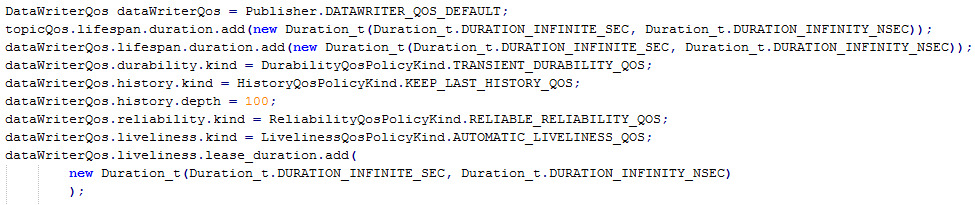
\includegraphics[width=\textwidth]{SettingQoSPublishers.png}
	\captionof{figure}{Setting the QoS parameters programatically}
\end{center}

\textbf{For DataReaders}
As seen on the following figure, a default QoS object is created and the custom values are then set. This is done in the main function in \textit{main.java} of the subscriber project and the object is then passed to the OfficeSubscriber constructor.
\begin{center}
	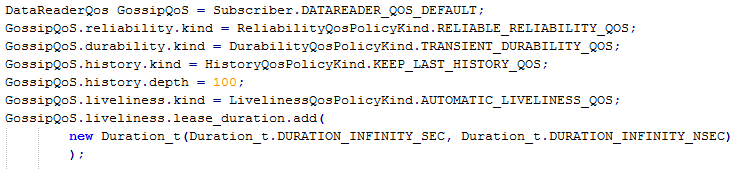
\includegraphics[width=\textwidth]{SettingQoSSubscribers.png}
	\captionof{figure}{Setting the QoS parameters programatically}
\end{center}

\section{Tests}
